\documentclass[aspectratio=169]{beamer}
\usepackage[utf8]{inputenc}
\usepackage[french]{babel}
\usepackage{graphicx}
\usepackage{booktabs}
\usepackage{xcolor}
\usepackage{subcaption}

\usetheme{Madrid}
\usecolortheme{dolphin}

\title[ERO2 - Moulinette]{Analyse et Optimisation de la Moulinette (ERO2)}
\subtitle{Modélisation, Simulation et Recommandations}
\author[Groupe ERO2]{Tanguy Ducrocq \and Quentin Gillet \and Luke Goboyan \and Pierre Lavielle \and Guillaume Rodriguez \and Louis Romain}
\date{\today}

\begin{document}

\begin{frame}
    \titlepage
\end{frame}

\begin{frame}{Plan de la présentation}
    \tableofcontents
\end{frame}

\section{Cadre Théorique}

\begin{frame}{Le Système Modélisé}
    Notre modèle se base sur un \textbf{Réseau de Jackson en tandem} composé de deux stations :
    \vspace{0.2cm}
    \begin{itemize}
        \item \textbf{Station 1 (Tests) :} File $M/M/3$ (3 serveurs).
        \item \textbf{Station 2 (Affichage) :} File $M/M/1$ (un seul serveur).
    \end{itemize}
    \vspace{0.2cm}
    \textbf{Hypothèses Mathématiques :}
    \begin{itemize}
        \item Arrivées selon un \textbf{processus de Poisson} (indépendance).
        \item \textbf{Théorème de Burke :} La sortie de la station 1 reste un processus de Poisson. Cela permet d'analyser les stations indépendamment.
    \end{itemize}
    \begin{figure}
        \centering
        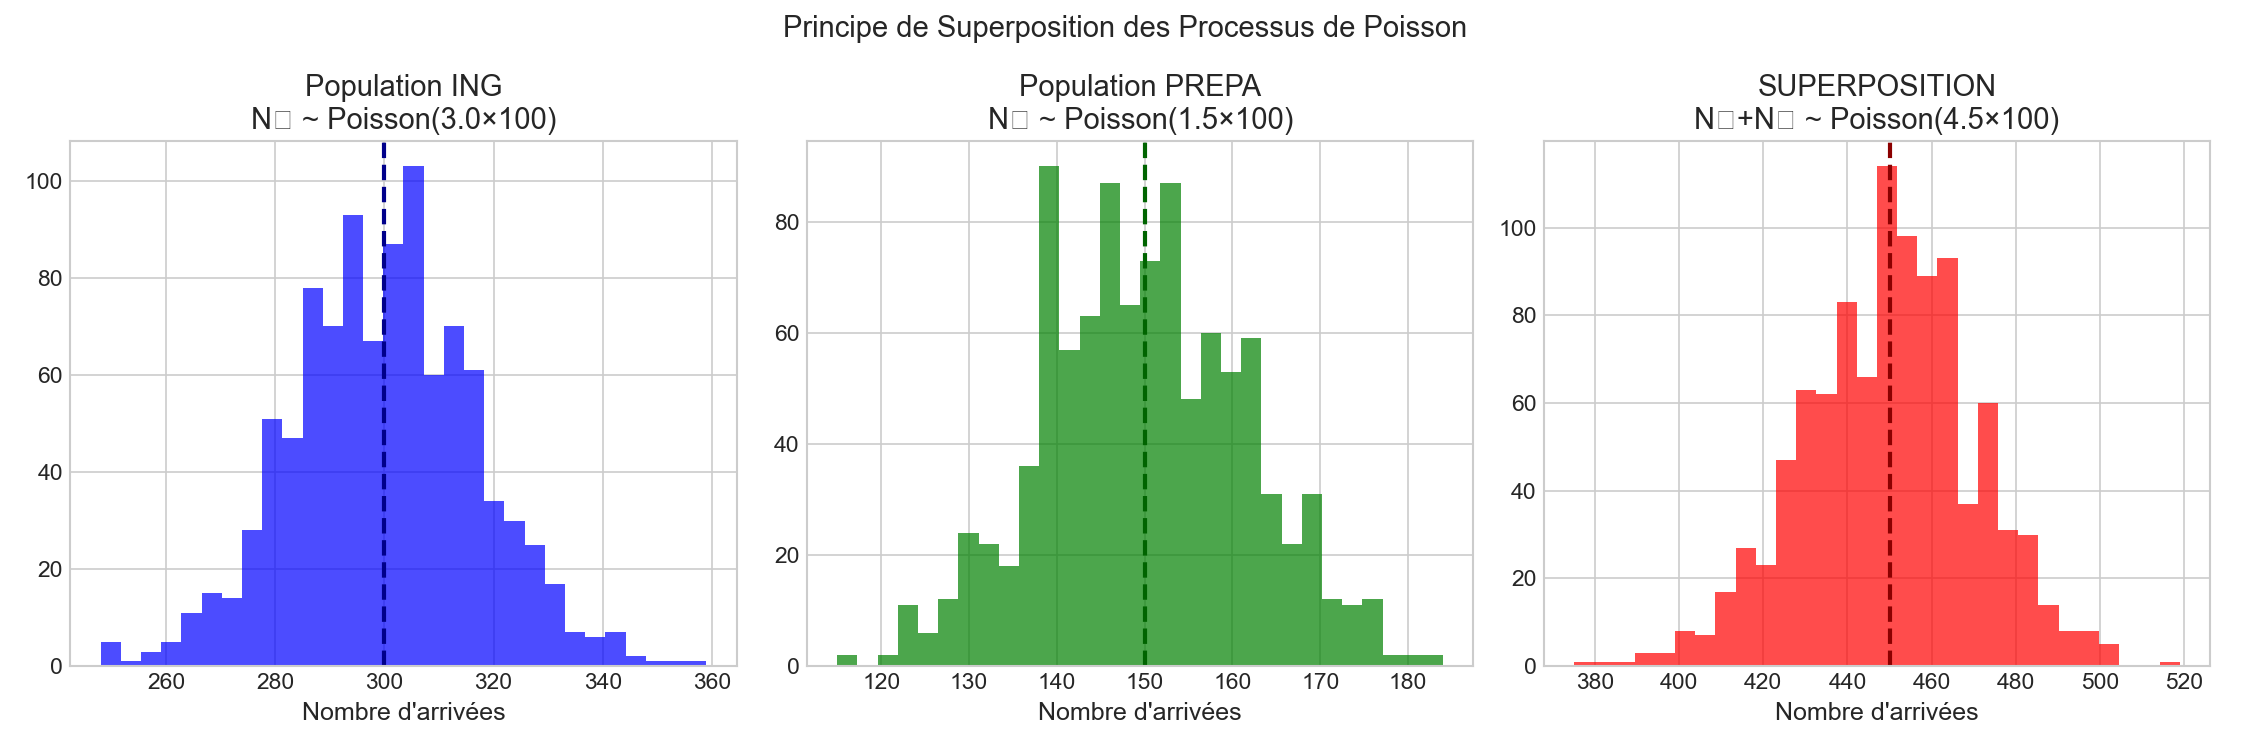
\includegraphics[width=0.45\textwidth]{img/generated/03_superposition_poisson.png}
        \caption{Validité des processus d'arrivée}
    \end{figure}
\end{frame}

\begin{frame}{Validation du Simulateur (Files Infinies)}
    Premier scénario (Waterfall) avec files infinies pour valider le modèle.
    \vspace{0.2cm}
    \begin{block}{Conformité Théorique}
        \begin{itemize}
            \item \textbf{Temps de séjour :} Erreur Simulation vs Théorie < 0.16\%.
            \item \textbf{Loi de Little ($L = \lambda \times W$)} : Écart constaté < 0.1\%.
        \end{itemize}
    \end{block}
    \begin{figure}
        \centering
        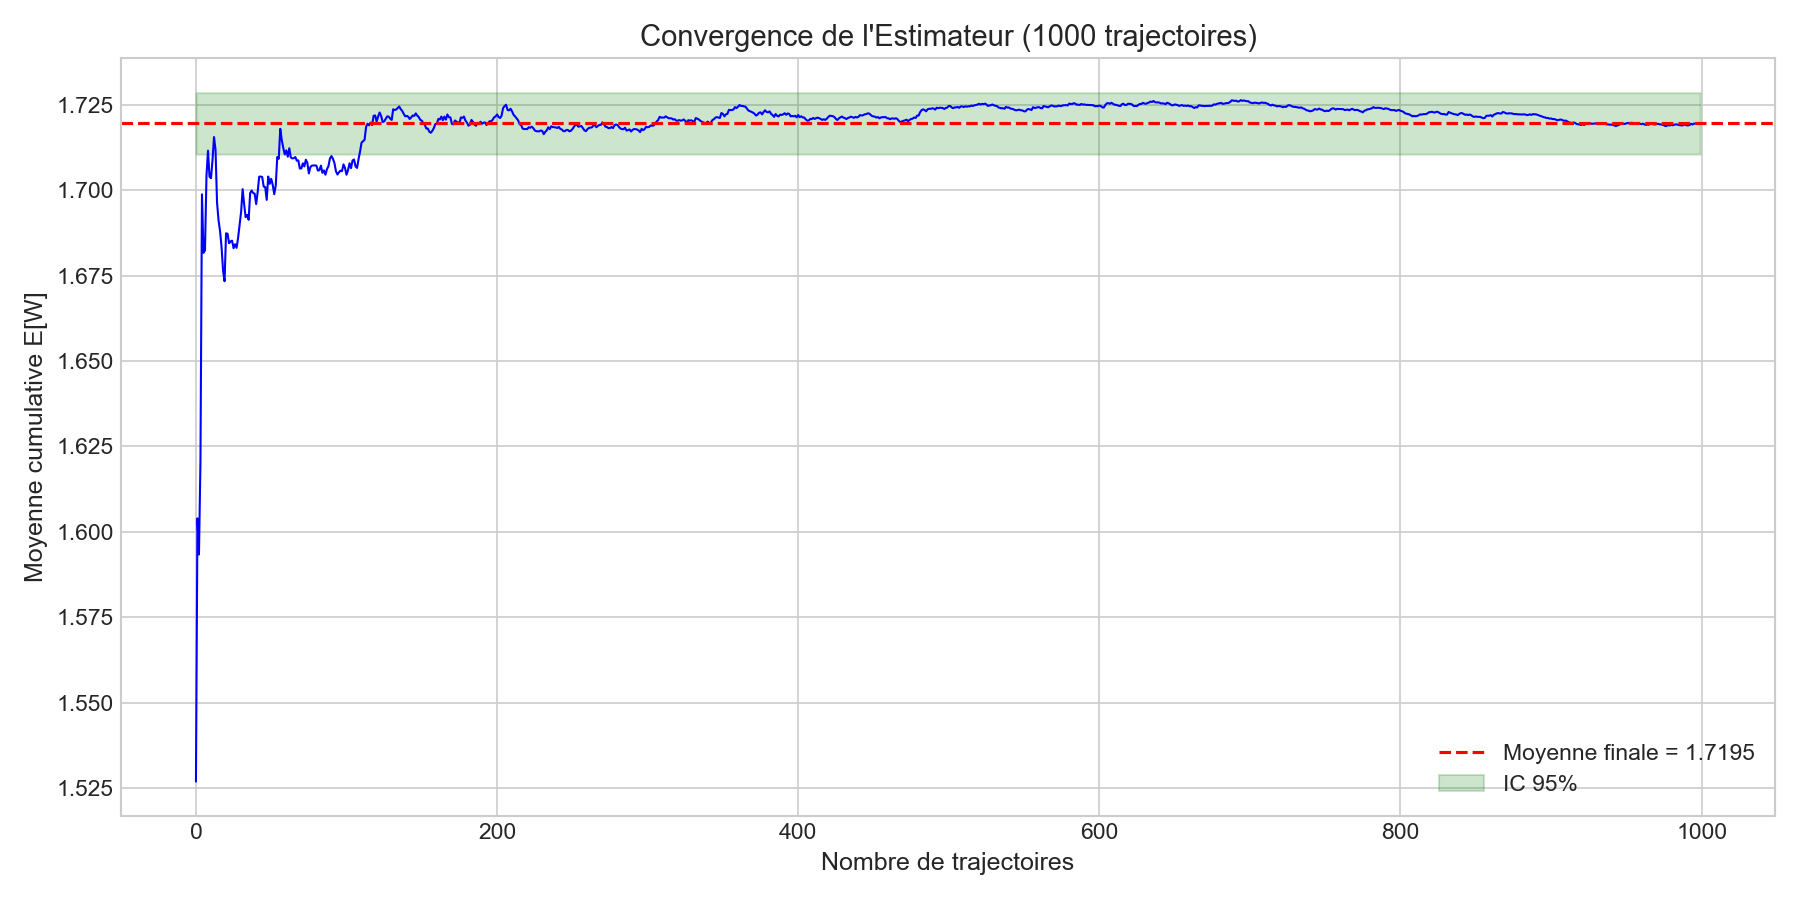
\includegraphics[width=0.55\textwidth]{img/generated/04_convergence_moyenne.png}
        \caption{Convergence du temps de séjour (Scénario idéal)}
    \end{figure}
\end{frame}

\section{Simulation 1: Files Finies}

\begin{frame}{Contraintes Réelles : Rejet vs Perte}
    Passage au modèle réel : Capacités physiques limitées ($k_s, k_f$).
    \vspace{0.2cm}
    \begin{itemize}
        \item \textbf{Rejet (File 1 pleine)} : Erreur immédiate, coût opérationnel faible.
        \item \textbf{Perte (File 2 pleine)} : "Page blanche". Risque critique : Calcul effectué mais résultat perdu (Gaspillage ressources).
    \end{itemize}
    \begin{figure}
        \centering
        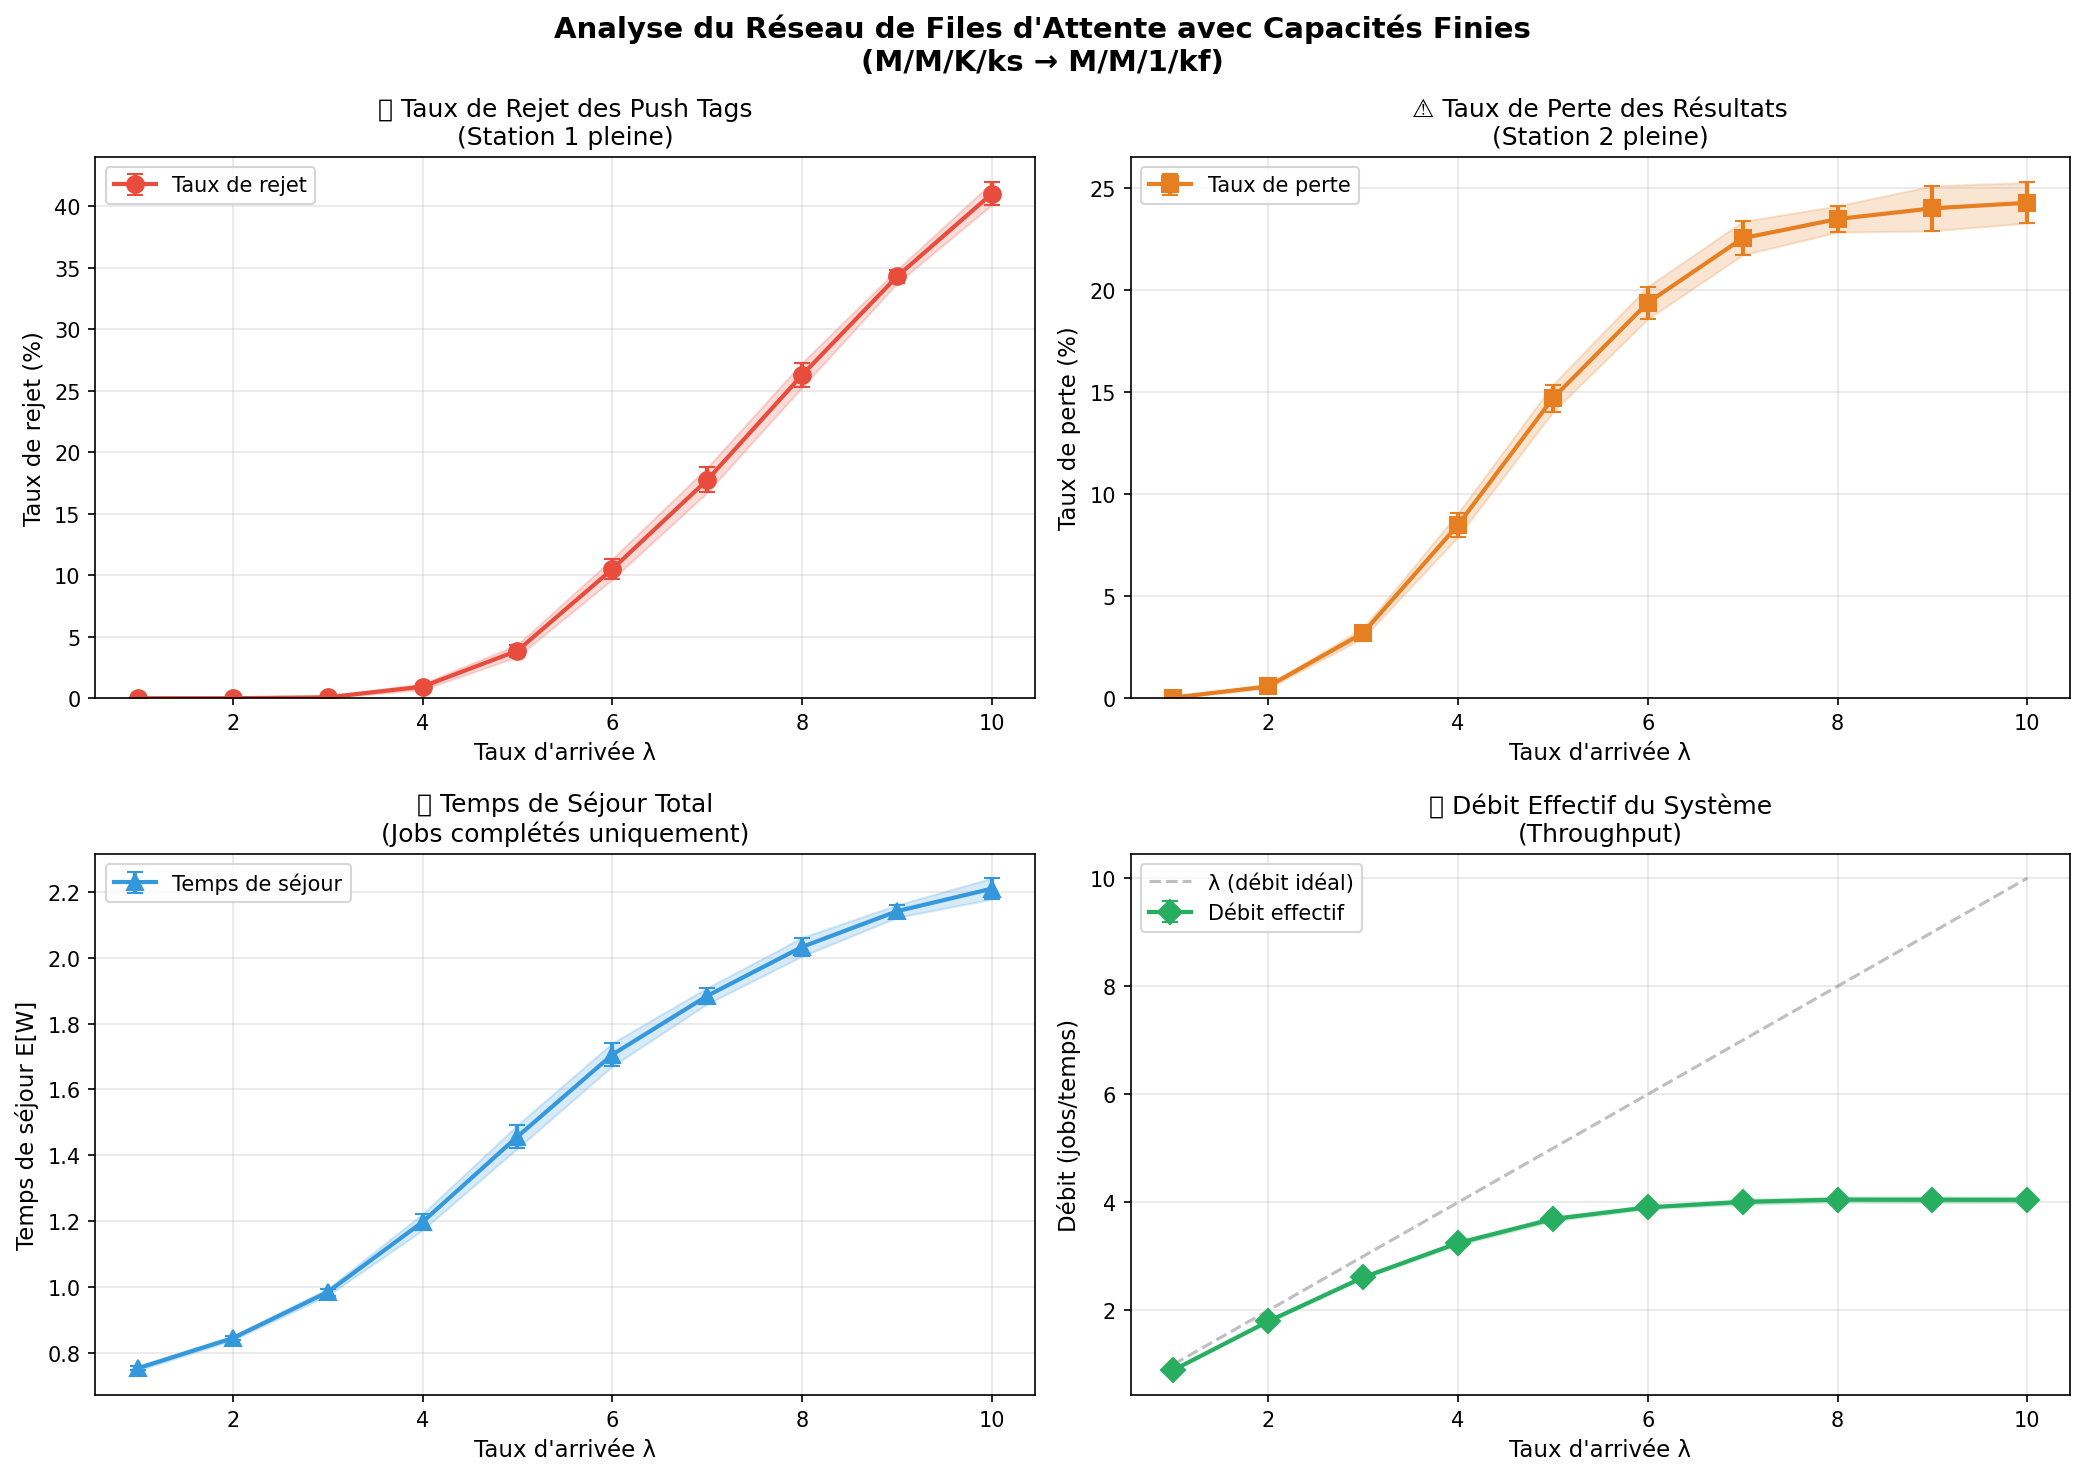
\includegraphics[width=0.6\textwidth]{img/queue_analysis.png}
        \caption{Dynamique d'occupation des files}
    \end{figure}
\end{frame}

\begin{frame}{Analyse de la Saturation \& Goulot}
    \begin{columns}
        \column{0.3\textwidth}
        \textbf{Saturation ($\lambda=6$)} :
        \begin{itemize}
            \item Près de \textbf{30\%} des soumissions en échec.
            \item Taux de perte ("pages blanches") $\approx$ \textbf{24\%}.
        \end{itemize}
        \vspace{0.5cm}
        \textbf{Le Goulot :}
        \begin{itemize}
            \item Débit effectif plafonne à \textbf{4 jobs/min}.
            \item C'est la \textbf{Station 2} ($M/M/1$).
        \end{itemize}

        \column{0.7\textwidth}
        \centering
        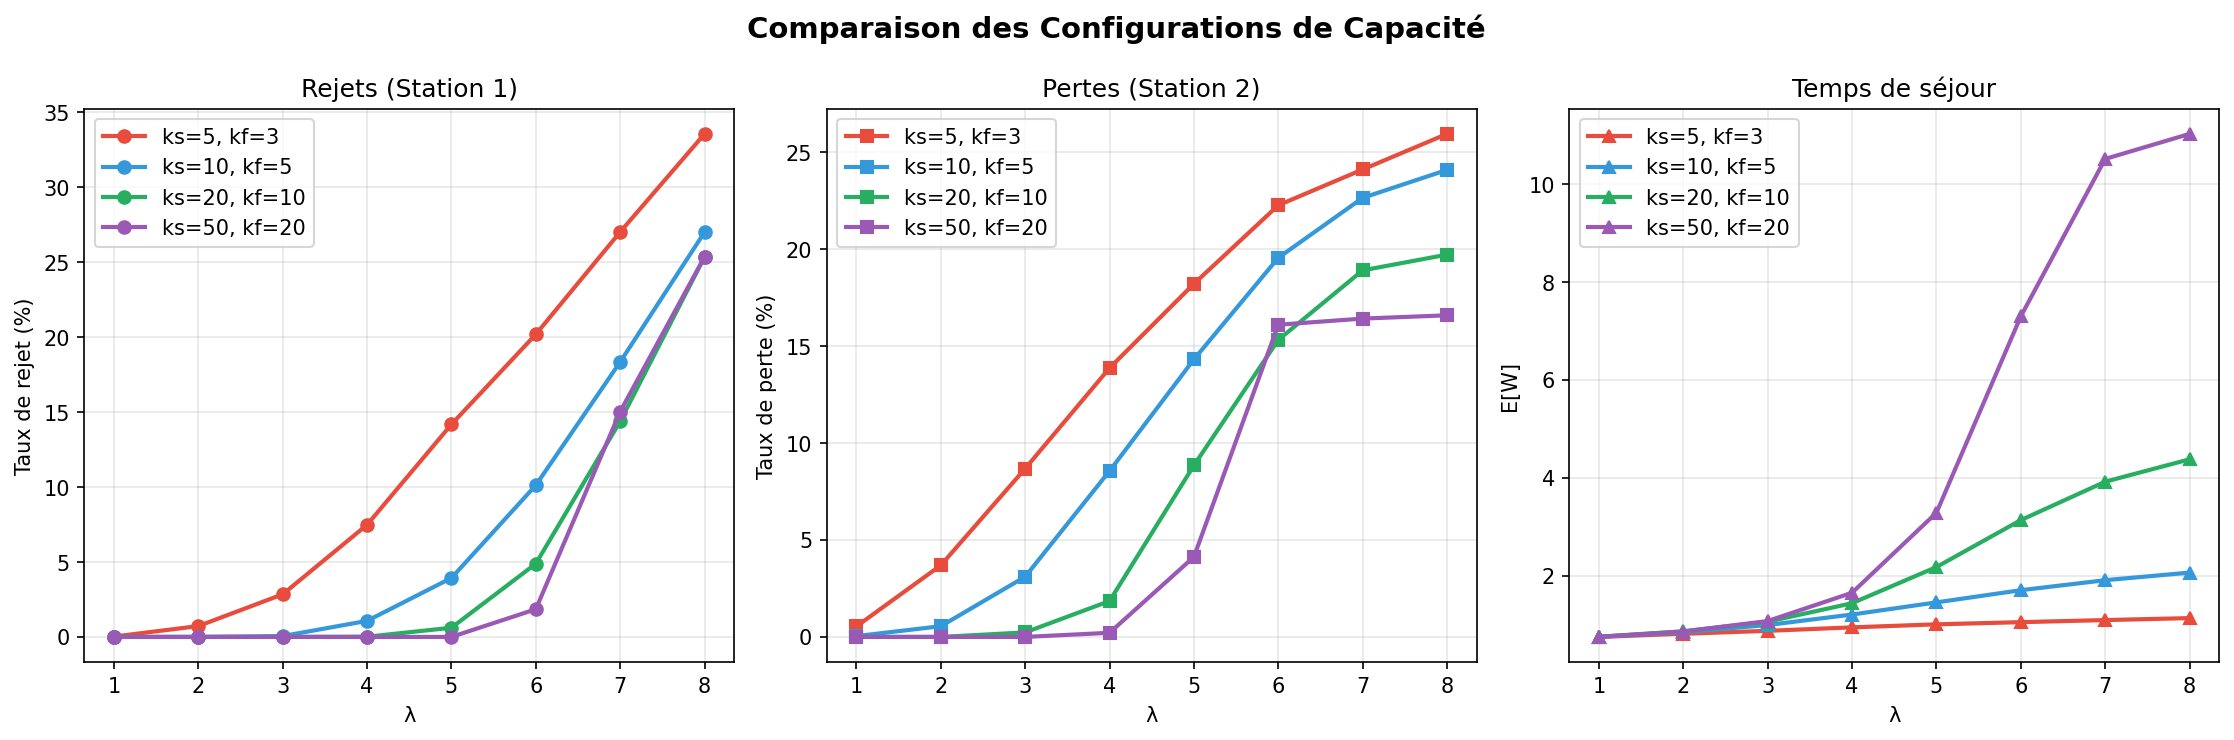
\includegraphics[width=\textwidth]{img/capacity_comparison.png}
    \end{columns}
\end{frame}

\section{Simulation 2: Backup}

\begin{frame}{Stratégie de Backup}
    \textbf{Objectif :} Éviter la perte sèche (page blanche) sauvant en tampon avant la file 2.
    \vspace{0.2cm}
    \begin{itemize}
        \item \textbf{Benchmark :} Comparaison de probabilités de backup ($p \in \{0, 0.25, 0.5, 0.75, 1\}$).
        \item \textbf{Compromis :} Le backup réduit la perte mais augmente le temps de séjour (plus de monde dans la file 2).
    \end{itemize}
    \begin{figure}
        \centering
        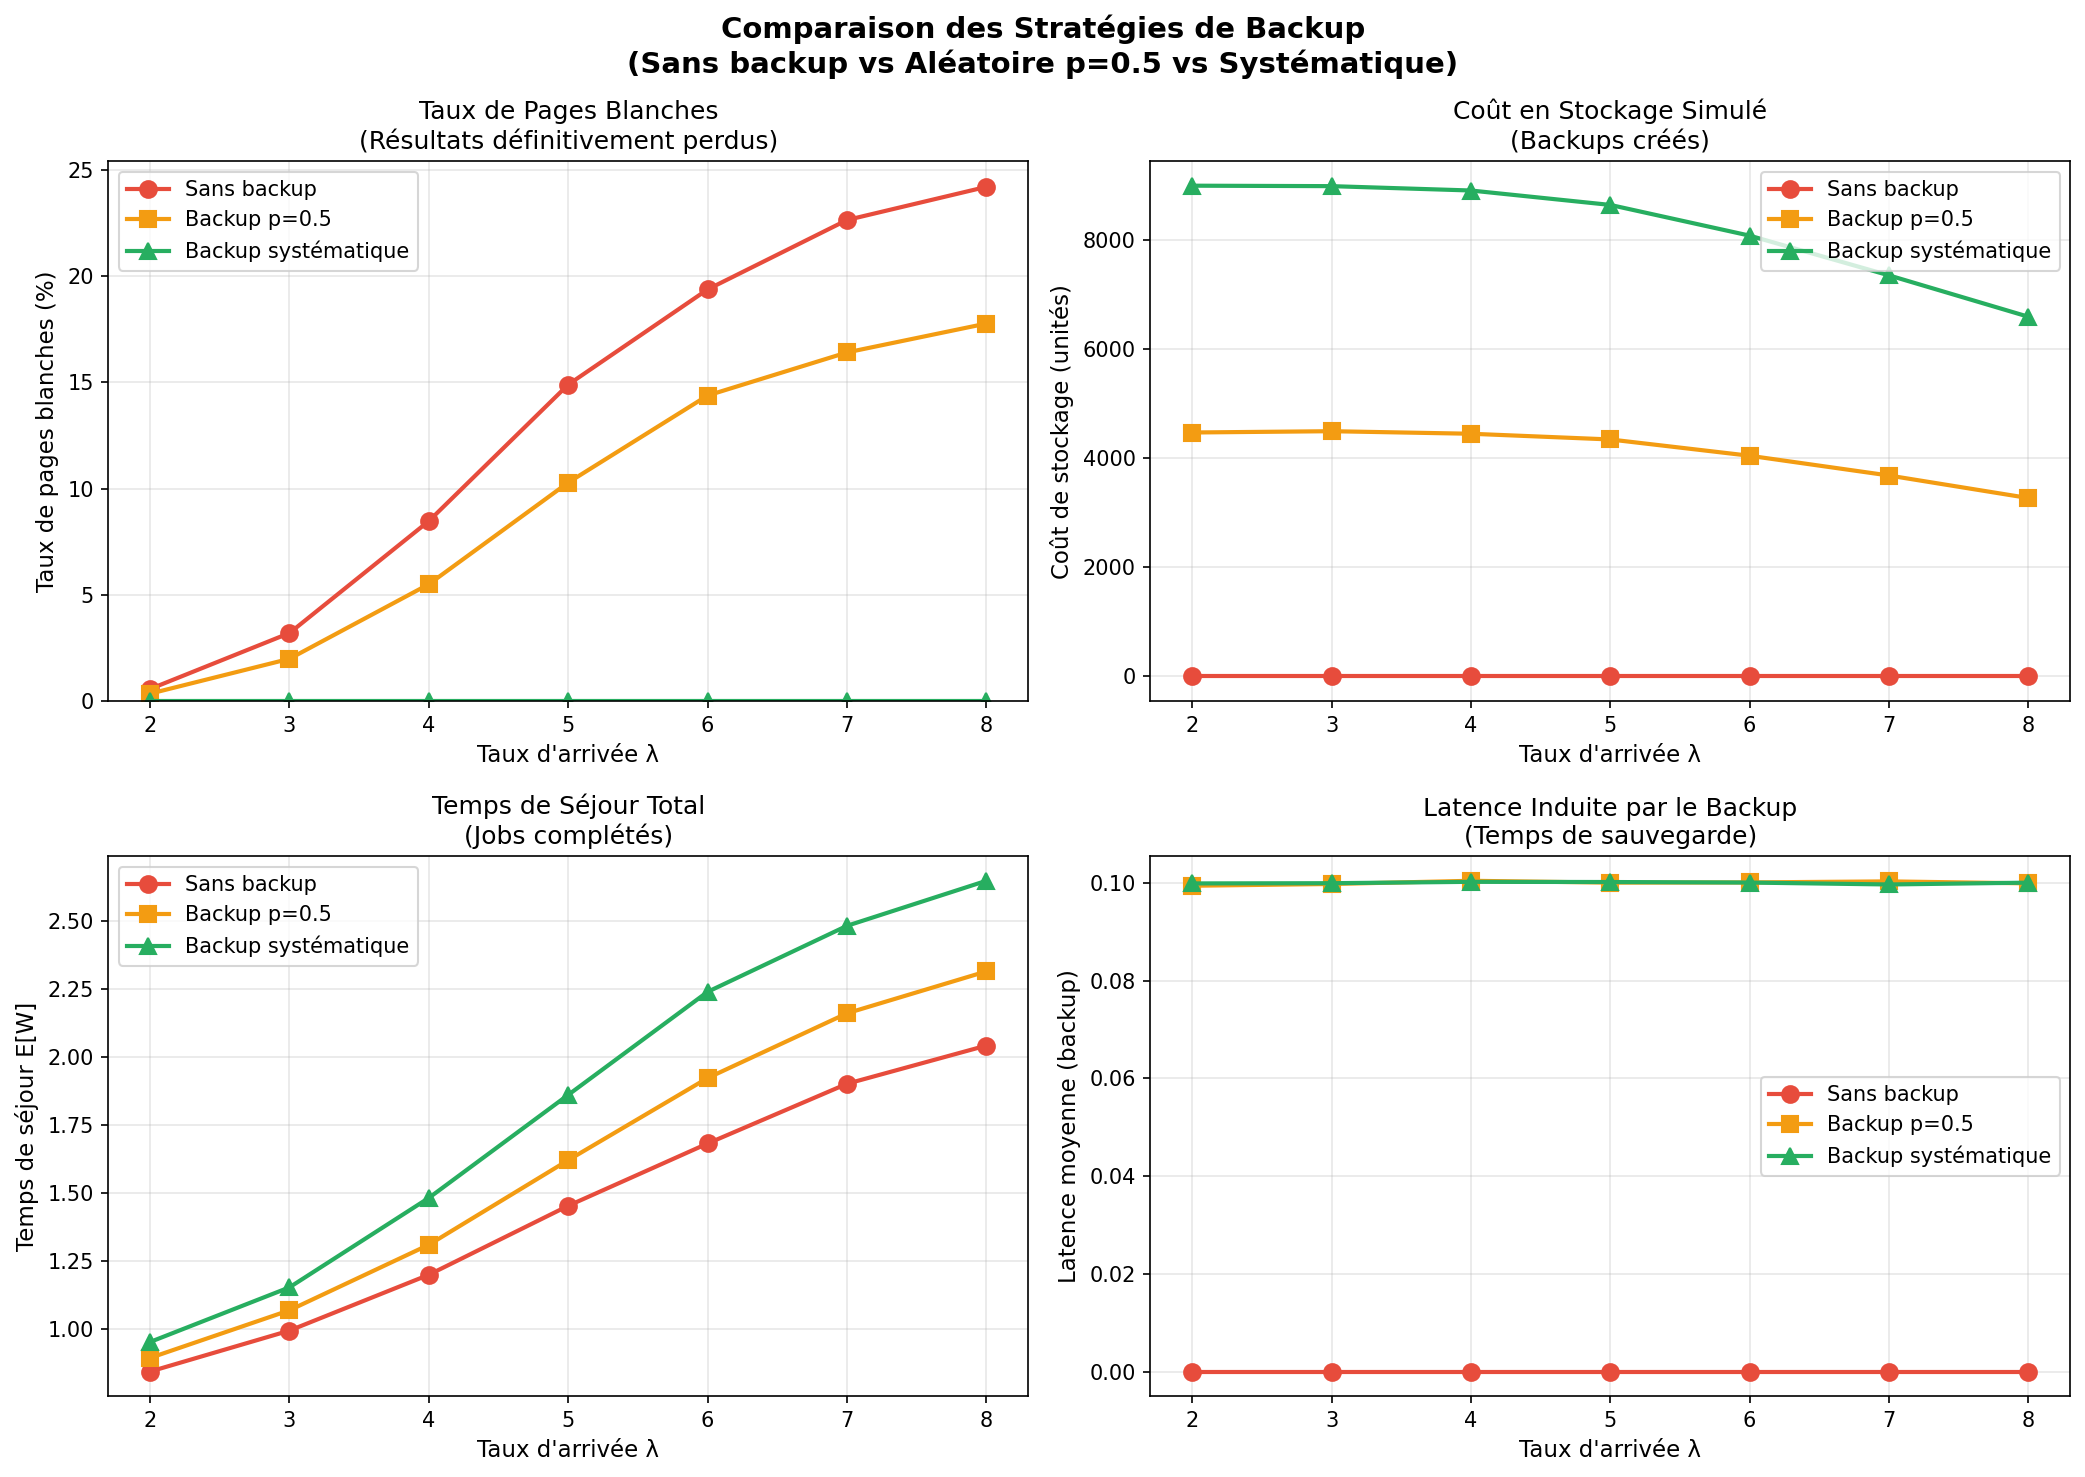
\includegraphics[width=0.5\textwidth]{img/backup_comparison.png}
        \caption{Compromis Temps/Perte en fonction de p}
    \end{figure}
\end{frame}

\begin{frame}{Optimisation : Le Gagnant}
    \begin{columns}
        \column{0.6\textwidth}
        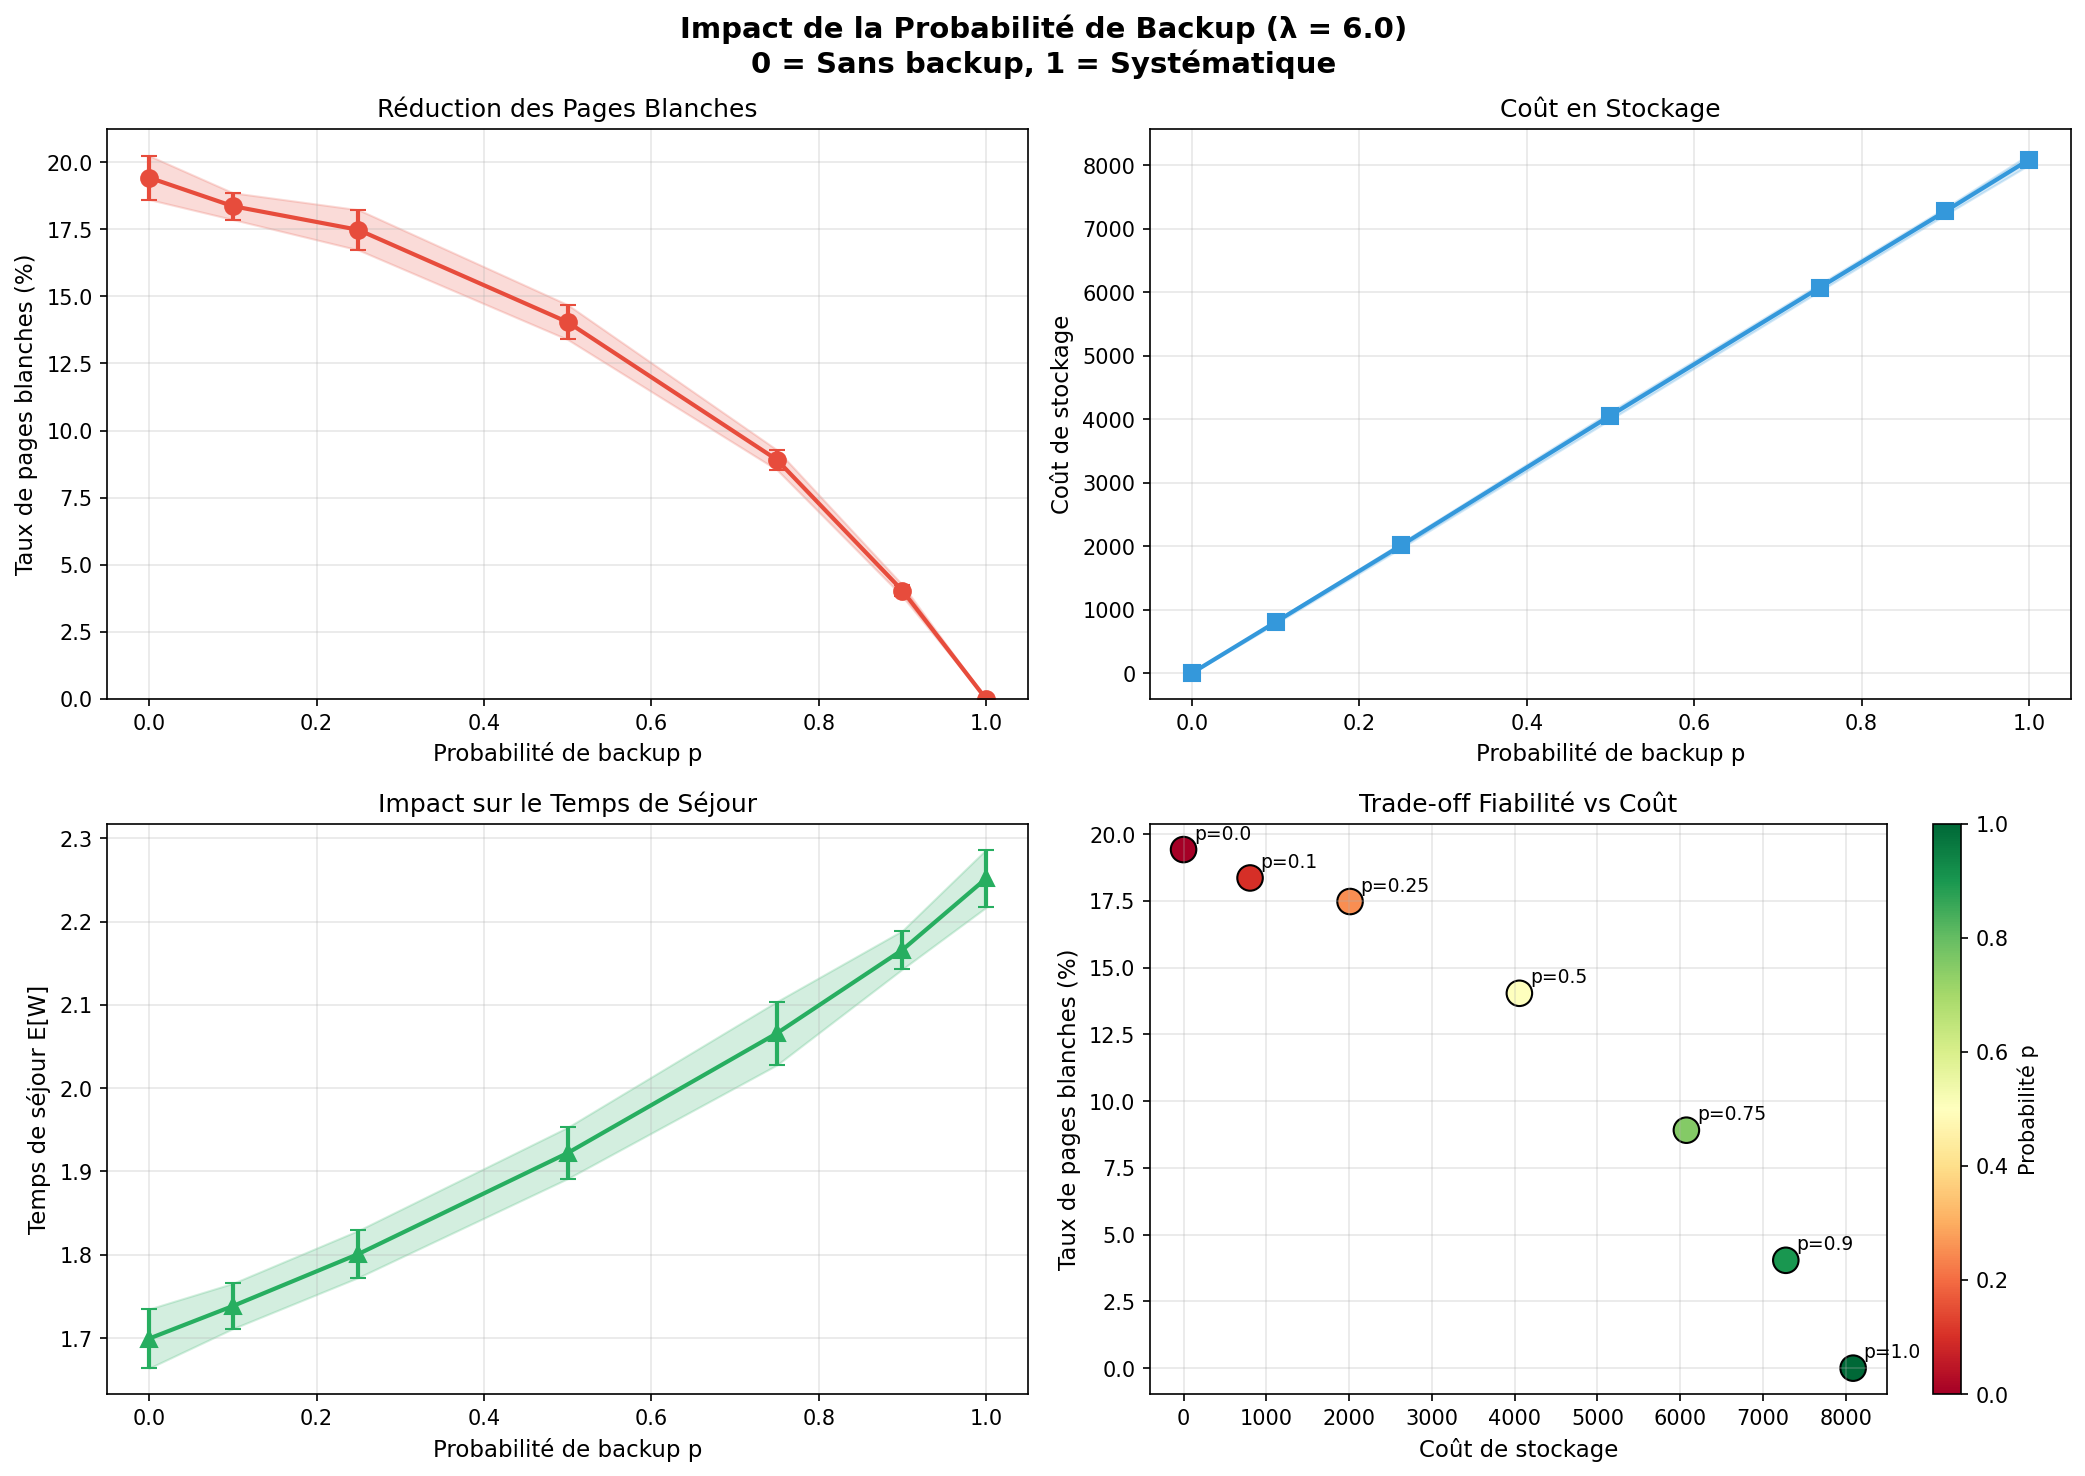
\includegraphics[width=\textwidth]{img/backup_probability_analysis.png}
        
        \column{0.4\textwidth}
        \textbf{Optimum : $p=0.5$}
        \begin{itemize}
            \item Réduction des pages blanches de \textbf{30\%}.
            \item Stockage divisé par 2 vs systématique.
            \item Coût temps négligeable ($+0.23$ min).
        \end{itemize}
    \end{columns}
\end{frame}

\section{Simulation 3: Multi-Populations}

\begin{frame}{ING vs PREPA : Inégalités}
    \textbf{Modélisation :}
    \begin{itemize}
        \item \textbf{ING} : Tests rapides ($\mu_1=4.0$).
        \item \textbf{PREPA} : Tests lents ($\mu_1=1.0$).
    \end{itemize}
    \vspace{0.2cm}
    \textbf{Constats :}
    \begin{itemize}
        \item Temps moyen : ING \textbf{2.84 min} vs PREPA \textbf{3.11 min}.
        \item Ratio $P/I = 1.10$ : Pénalité structurelle de 10\% pour les débutants.
    \end{itemize}
\end{frame}

\begin{frame}{Visualisation des Populations}
    \begin{figure}
        \centering
        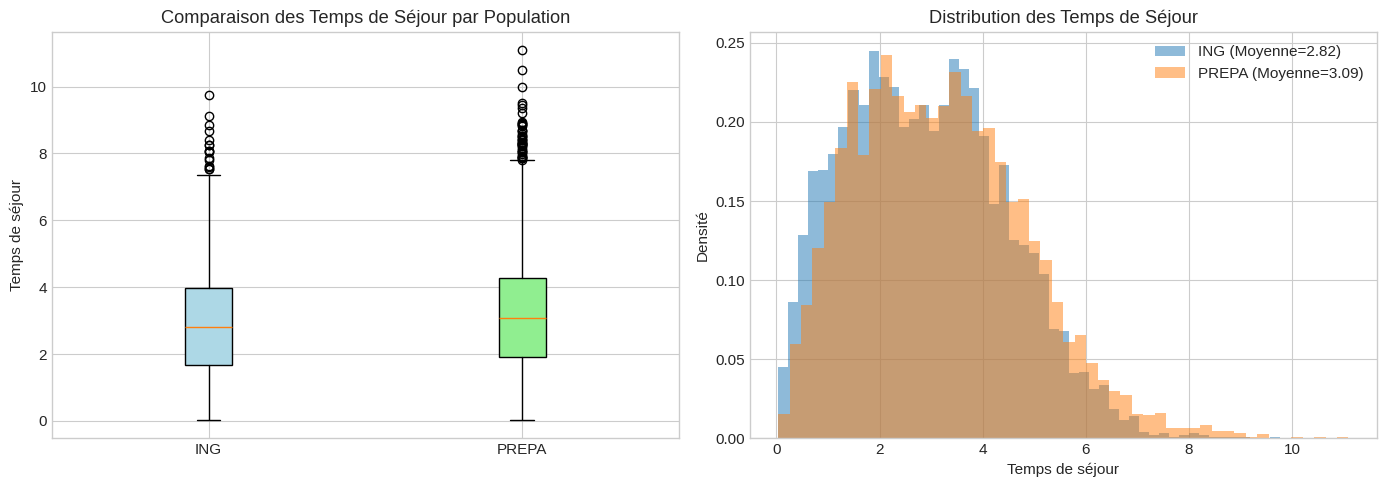
\includegraphics[width=0.7\textwidth]{img/generated/02_comparaison_populations.png}
        \caption{Distribution des temps par population}
    \end{figure}
\end{frame}

\section{Simulation 4: Blocage}

\begin{frame}{La Fausse Bonne Idée : Throttling}
    \textbf{Mécanisme :} Blocage périodique ($t_{block}$) pour réguler.
    \begin{itemize}
        \item Disponibilité système : \textbf{33.3\%} du temps seulement.
    \end{itemize}
    \vspace{0.5cm}
    \textbf{Le Paradoxe de l'Équité :}
    \begin{itemize}
        \item (+) Ratio équité $P/I \approx 1.01$.
        \item \textbf{(-) Désastre Performance :} Temps de séjour explosent de \textbf{900\%}.
    \end{itemize}
\end{frame}

\begin{frame}{Impact du Blocage : Performance}
    Graphique montrant l'explosion des temps de séjour quand le blocage s'active.
    \begin{figure}
        \centering
        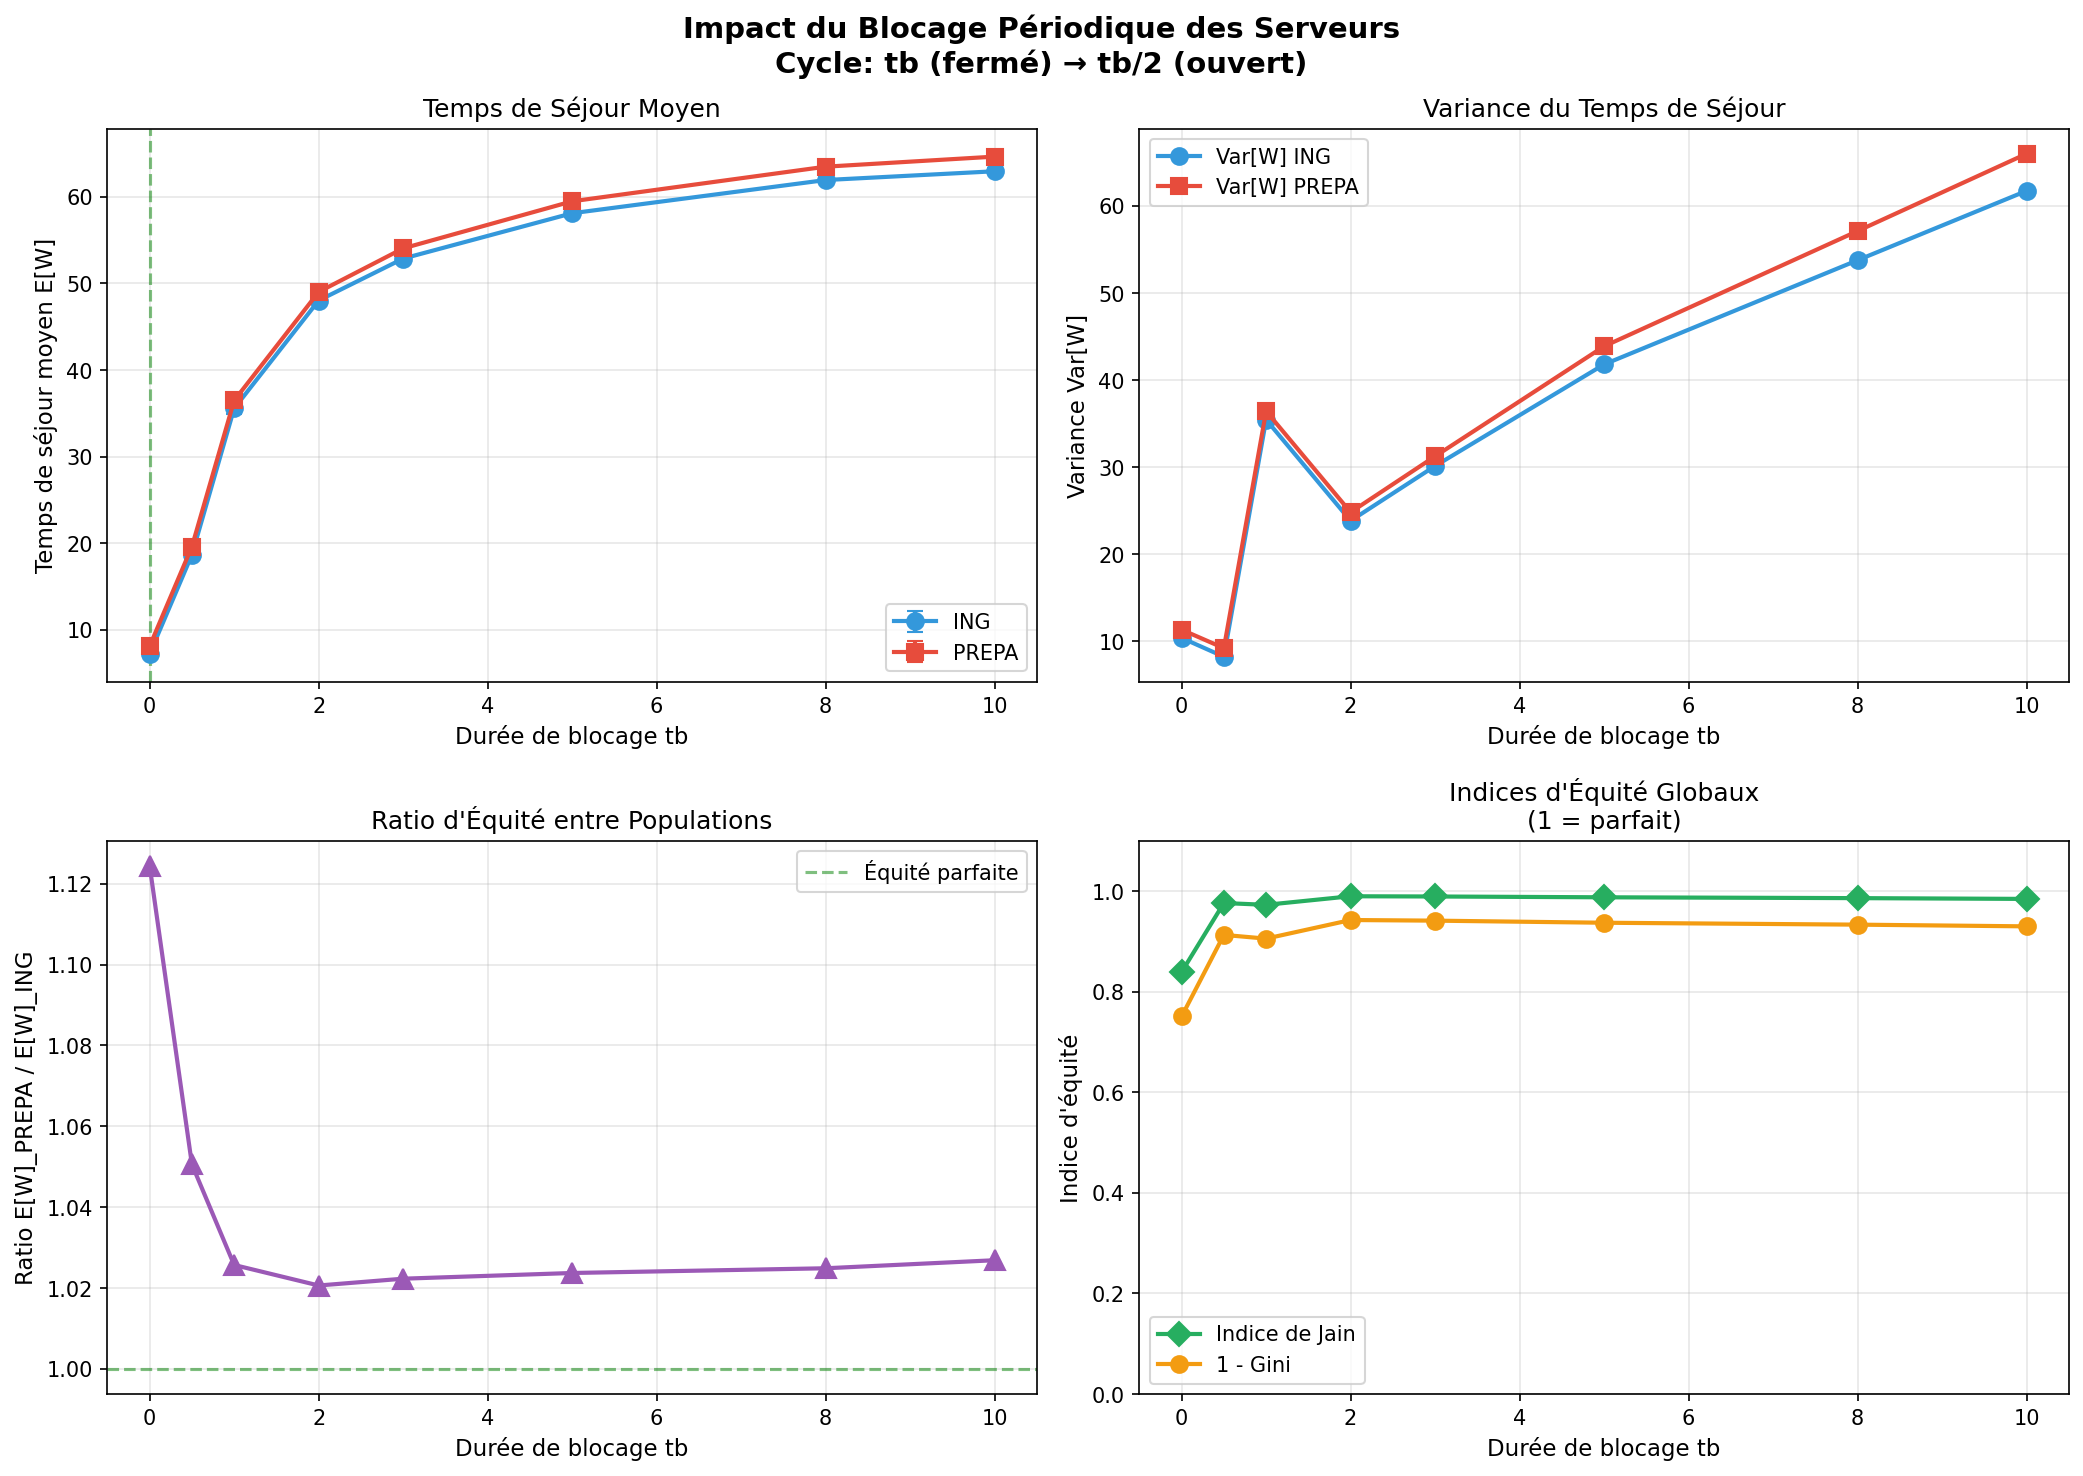
\includegraphics[width=0.7\textwidth]{img/blocking_comparison.png}
        \caption{Temps de séjour en fonction du temps de blocage}
    \end{figure}
\end{frame}

\begin{frame}{Impact du Blocage : Équité}
    Graphique confirmant que l'équité s'améliore (Coefficient de Gini baisse), mais à quel prix ?
    \begin{figure}
        \centering
        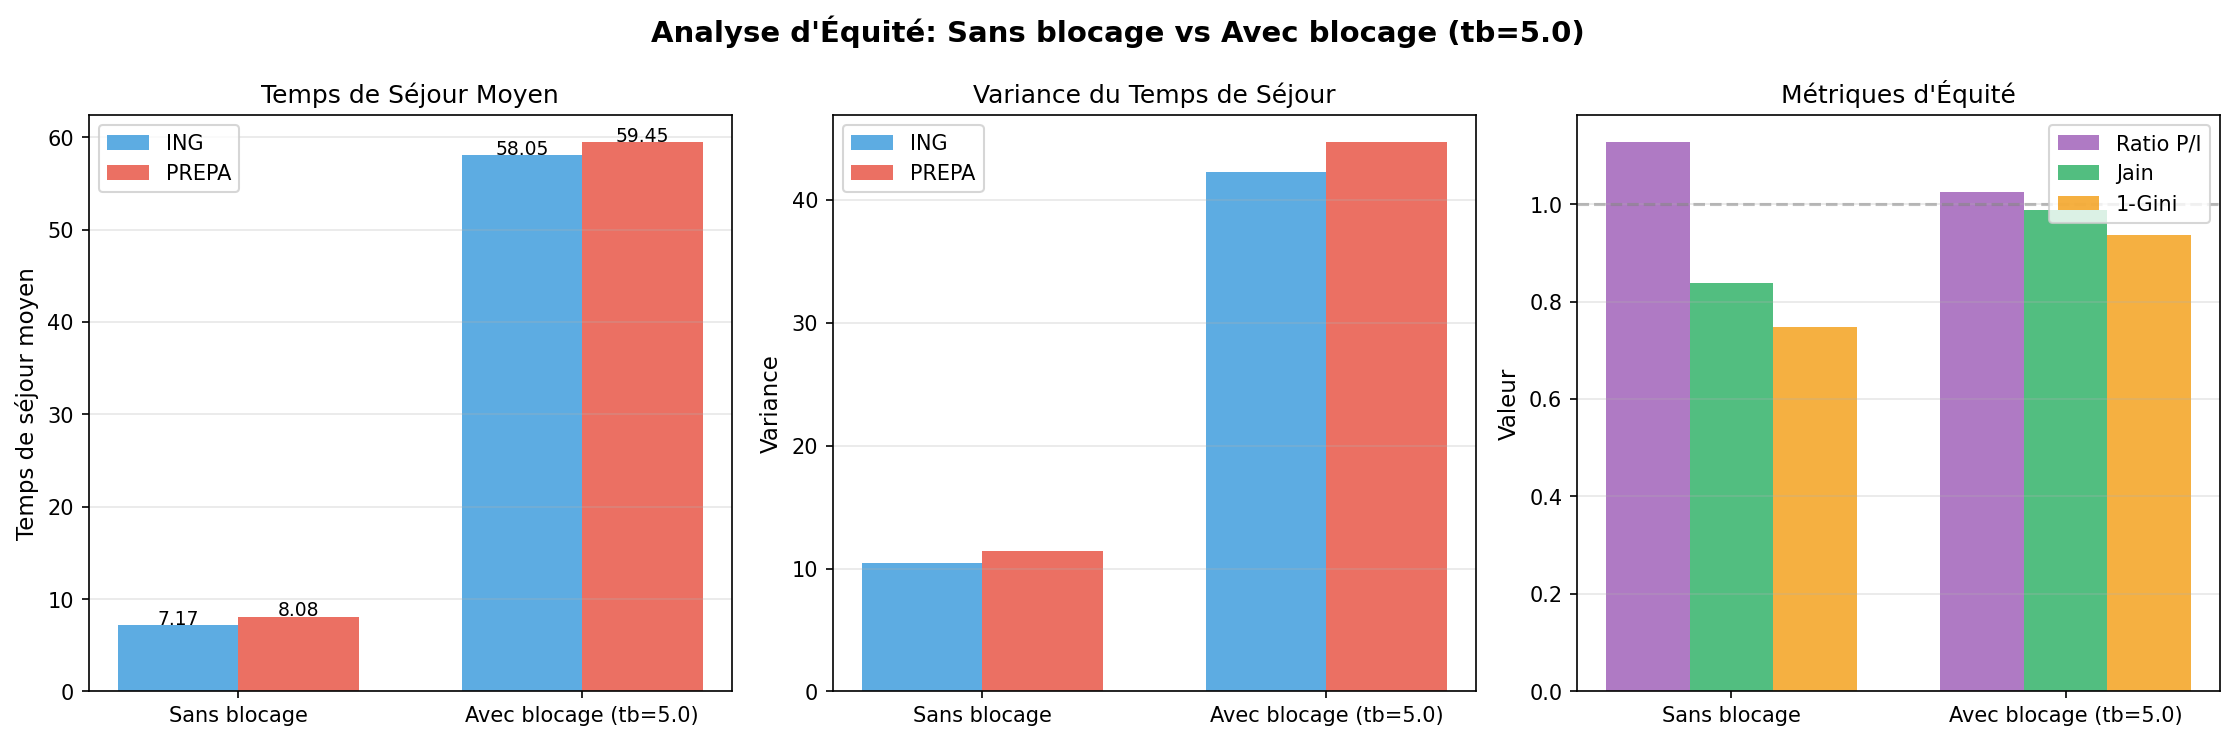
\includegraphics[width=0.7\textwidth]{img/fairness_analysis.png}
        \caption{Analyse de l'indice de Gini (Inégalité)}
    \end{figure}
\end{frame}

\section{Optimisation \& Conclusion}

\begin{frame}{Politiques de Priorité}
    Comparatif des algorithmes pour le compromis Équité/Performance :
    \vspace{0.2cm}
    \begin{table}
        \centering
        \begin{tabular}{l l l}
            \toprule
            Politique & Performance & Équité \\
            \midrule
            FCFS & Standard & Iniquité (Ratio 1.77) \\
            SRPT & \textcolor{green}{Meilleur (1.15)} & \textcolor{red}{Désastreux (Ratio 3.31)} \\
            \textbf{PREPA\_FIRST} & \textcolor{blue}{Bon (1.57)} & \textcolor{green}{Excellent (Ratio 1.08)} \\
            \bottomrule
        \end{tabular}
    \end{table}
    \vspace{0.2cm}
    $\rightarrow$ \textbf{PREPA\_FIRST} est la meilleure discrimination positive.
\end{frame}

\begin{frame}{Pourquoi PREPA\_FIRST ? (Preuve Graphique)}
    L'étude des ratios montre que c'est la seule politique qui stabilise les inégalités à forte charge.
    \begin{figure}
        \centering
        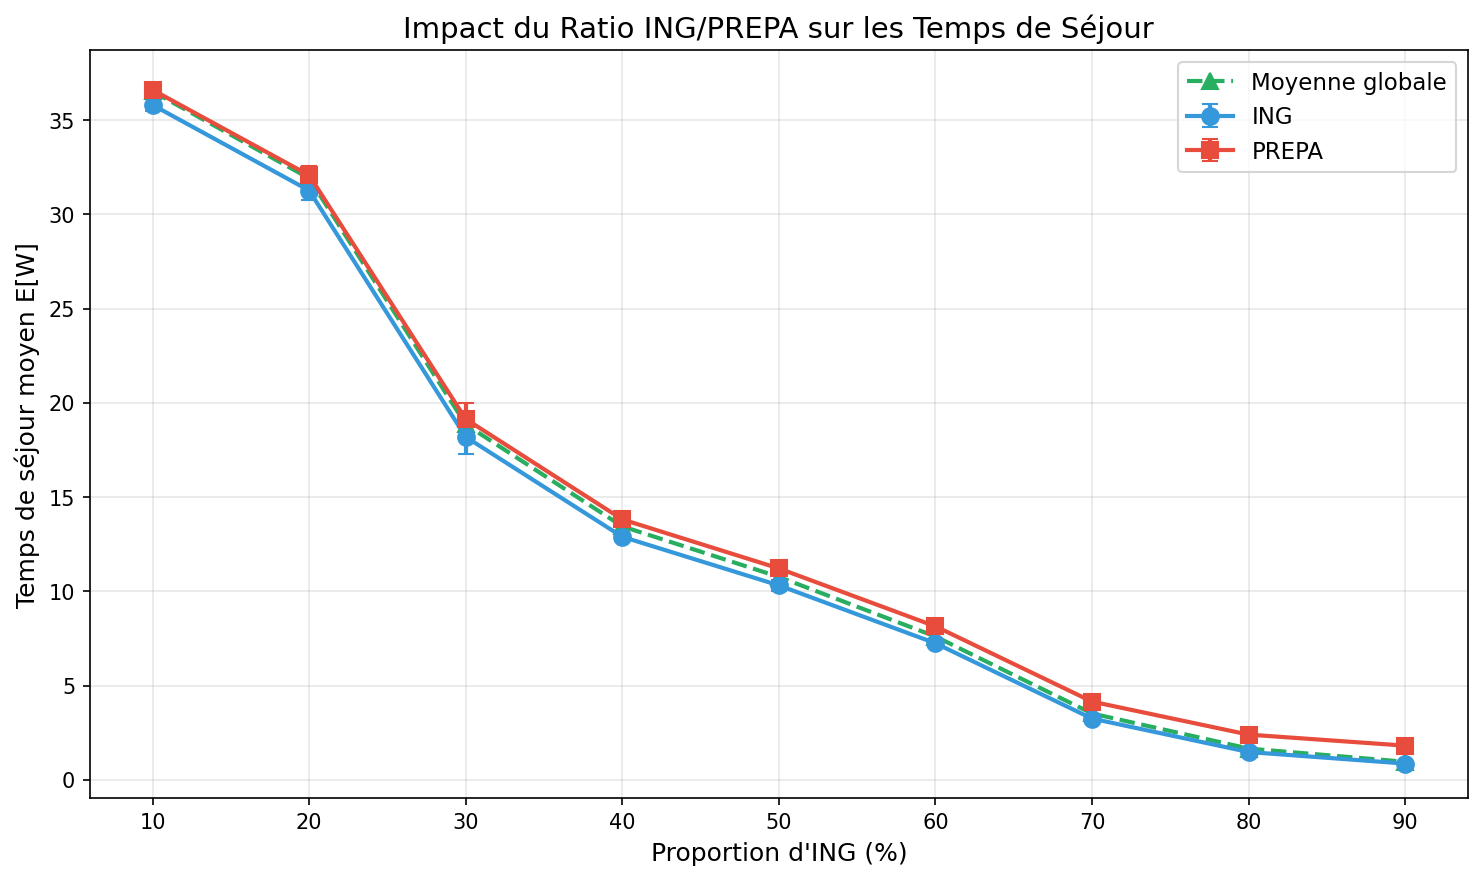
\includegraphics[width=0.6\textwidth]{img/ratio_study.png}
        \caption{Ratio Temps Prépa / Temps Ingénieur selon la politique}
    \end{figure}
\end{frame}

\begin{frame}{Plan d'Action (Recommandations)}
    \begin{columns}
        \column{0.6\textwidth}
        \textbf{1. Augmenter $k_f$ (5 $\rightarrow$ 10)}
        \begin{itemize}
            \item \textbf{Gain :} Réduit les pertes ("pages blanches") de 60\%.
            \item \textbf{Analyse Coût/Bénéfice :} Investissement prioritaire (Station 2), coût infrastructure faible pour un gain critique.
        \end{itemize}
        \vspace{0.3cm}
        \textbf{2. Backup Aléatoire ($p=0.5$)}
        \begin{itemize}
            \item \textbf{Gestion du Risque :} Sécurise les données restantes.
            \item \textbf{Compromis :} Faible coût stockage/temps pour une résilience maximale.
        \end{itemize}
        \vspace{0.3cm}
        \textbf{3. Politique PREPA\_FIRST}
        \begin{itemize}
            \item \textbf{Coût Social :} Rétablit l'équité sans impact majeur sur la performance globale.
        \end{itemize}

        \column{0.4\textwidth}
        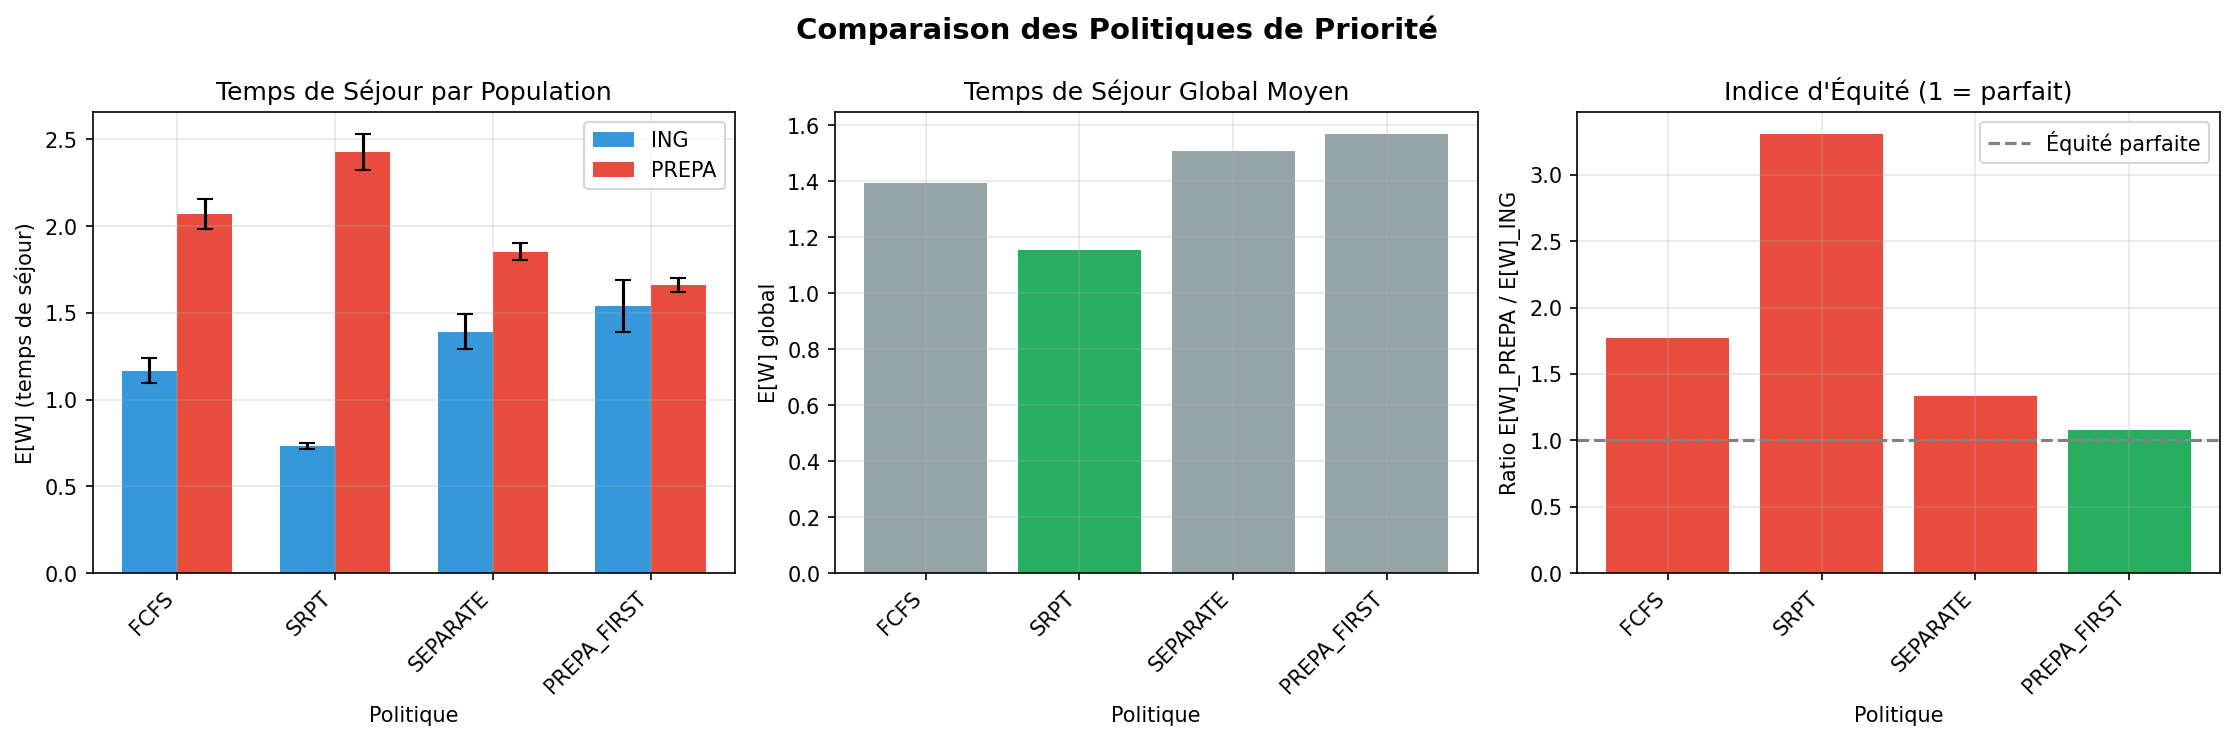
\includegraphics[width=\textwidth]{img/policy_comparison.png}
    \end{columns}
\end{frame}

\begin{frame}
    \centering
    \Huge \textbf{Merci de votre attention.}
    \vspace{1cm}
    \\
    \large Groupe ERO2
\end{frame}

\end{document}
